%	proofeg.tex	(An example file for proof.sty)
%
%		Mar 6, 1997
%		Makoto Tatsuta
%
%	I hope you can learn how to use proof figure macros easily
%	by these examples.


\def\imp{\to}
\def\land{\mathbin\&}
% for LaTeX 2e naitive mode.
\documentclass[]{article}
\usepackage{proof}
\usepackage{tikz}
\usetikzlibrary{trees}

\begin{document}

\section{Semantic Tableaux}
\textbf{a)} From the open leaves of the tableau we see that there are the following models that satisfy the formula $(p\rightarrow q) \rightarrow r$: $\{
\{(p\rightarrow F), (q, \rightarrow F), (r\rightarrow T)\},
\{(p\rightarrow F), (q, \rightarrow T), (r\rightarrow T)\},
\{(p\rightarrow T), (q, \rightarrow F), (r\rightarrow F)\},
\{(p\rightarrow T), (q, \rightarrow F), (r\rightarrow T)\},
\{(p\rightarrow T), (q, \rightarrow T), (r\rightarrow T)\}
\}$. In the set of propositions $P = \{p, q, r\}$, the
formula $(\neg p \rightarrow r) \wedge (q \rightarrow r)$ has the same models $M((p\rightarrow q) \rightarrow r) = M((\neg p \rightarrow r) \wedge (q \rightarrow r))$. Therefore, we conclude that $(p\rightarrow q) \rightarrow r$ and $(\neg p \rightarrow r) \wedge (q \rightarrow r)$ are logically equivalent.

\begin{figure}[h]
\centering
\begin{tikzpicture}[level distance=1.5cm,
  level 1/.style={sibling distance=3cm},
  level 2/.style={sibling distance=1.5cm}]
  \node {$(p\rightarrow q) \rightarrow r$}
    child {node {$\neg (p \rightarrow q)$}
      child {node {$p, \neg q$}}
    }
    child {node {$r$}};
\end{tikzpicture}
\caption{Left-hand side} \label{fig:LHS}
\end{figure}

\begin{figure}[h]
\centering
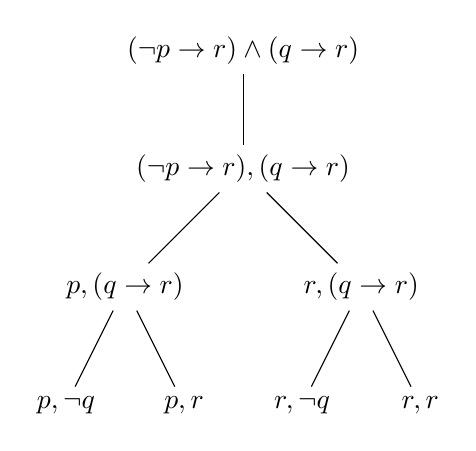
\begin{tikzpicture}[level distance=1.5cm,
  level 1/.style={sibling distance=3cm},
  level 3/.style={sibling distance=1.5cm}]
  \node {$(\neg p \rightarrow r) \wedge (q \rightarrow r)$}
    child {node {$(\neg p \rightarrow r),(q \rightarrow r)$}
      child {node {$p, (q\rightarrow r)$}
    	child {node {$p, \neg q$}}
   	    child {node {$p, r$}}
      }    	
      child {node {$r, (q\rightarrow r)$}
    	child {node {$r, \neg q$}}
   	    child {node {$r, r$}}      
      }
    };
\end{tikzpicture}
\caption{Right-hand side} \label{fig:RHS}
\end{figure}

\noindent \textbf{b)} To show that $(((p \rightarrow (q \wedge r)) \lor ((q \wedge r) \rightarrow p))\rightarrow p)$ is falsifiable, we must show that there exist models for the inverse, namely $\neg (((p \rightarrow (q \wedge r)) \lor ((q \wedge r) \rightarrow p))\rightarrow p)$. The semantic tableaux of the inverse can be found in Figure \ref{fig:both}. Two examples of interpretations which yield false are: $\{\{(p\rightarrow F), (q\rightarrow T), (r\rightarrow T)\},\{(p\rightarrow F),(q\rightarrow F),(r\rightarrow F)\}\}$


\begin{figure}[h]
\centering
\begin{tikzpicture}[level distance=1.5cm,
  level 1/.style={sibling distance=8cm},
  level 3/.style={sibling distance=5cm},
  level 4/.style={sibling distance=1.5cm}]
  \node {$\neg (((p \rightarrow (q \wedge r)) \lor ((q \wedge r) \rightarrow p))\rightarrow p)$}
    child {node {$(p \rightarrow (q \wedge r)) \lor ((q \wedge r) \rightarrow p), \neg p$}
      child {node {$p \rightarrow (q \wedge r), \neg p$}
    	child {node {$ \neg p, \neg p$}}
   	    child {node {$q \wedge r, \neg p$}
    	  child {node {$q,r, \neg p$}}
   	    }
      }    	
      child {node {$(q \wedge r) \rightarrow p, \neg p$}
    	child {node {$\neg (q \wedge r), \neg p$}
		  child {node {$\neg q, \neg p$}}
		  child {node {$\neg r, \neg p$}}
    	}
   	    child {node {$p, \neg p$}}      
      }
    };
\end{tikzpicture}
\caption{Semantic Tableaux for $\neg (((p \rightarrow (q \wedge r)) \lor ((q \wedge r) \rightarrow p))\rightarrow p)$} \label{fig:both}
\end{figure}

\section{Logical Equivalence}
$$
\infer[(L_\leftrightarrow)]{\Gamma, \phi \leftrightarrow \psi\vdash\Delta}{\Gamma, \phi \rightarrow \psi, \psi \rightarrow \phi\vdash\Delta}
$$

$$
\infer[(R_\leftrightarrow)]{\Gamma\vdash\Delta, \phi \leftrightarrow \psi}{
\Gamma \vdash \Delta, \phi \rightarrow \psi
&
\Gamma \vdash \Delta, \psi \rightarrow \phi
}
$$

$$
\infer[R_\rightarrow]{\vdash ((p \leftrightarrow q) \wedge (q \leftrightarrow r)) \rightarrow (r \leftrightarrow p)}{
	\infer[L_\wedge]{((p \leftrightarrow q) \wedge (q \leftrightarrow r)) \vdash (r \leftrightarrow p)}{
		\infer[L_\leftrightarrow]{(p \leftrightarrow q), (q \leftrightarrow r) \vdash (r \leftrightarrow p)}{	
			\infer[L_\leftrightarrow]{(p \rightarrow q),(q \rightarrow p), (q \leftrightarrow r) \vdash (r \leftrightarrow p)}{		
				\infer[L_\leftrightarrow]{(p \rightarrow q),(q \rightarrow p), (q \rightarrow r),(r \rightarrow q) \vdash (r \leftrightarrow p)}{					
				}			
			}				
		}
	}
}
$$
\section{Gentzen}

\section{Hilbert}













\end{document}
